\documentclass[11pt,a4paper]{article}
\usepackage[utf8]{inputenc}
\usepackage{graphicx}
\usepackage{xcolor}
\usepackage{hyperref}
\usepackage{geometry}
\usepackage{titlesec}
\usepackage{enumitem}
\usepackage{fontawesome}
\usepackage{tikz}
\usepackage{float}
\usepackage{pgfplots}
\pgfplotsset{compat=1.16}
\usetikzlibrary{positioning,calc}
\usepackage{amsmath}
\usepackage{tcolorbox}
\usepackage{avant}
\usepackage{microtype}
\usepackage{sectsty}
\usepackage{fancyhdr}
\usepackage{titling}
\usepackage{multicol}

% Simplified color scheme - fewer colors
\definecolor{fabPrimary}{RGB}{0, 0, 0}           % Black
\definecolor{fabAccent}{RGB}{212, 175, 55}       % Gold
\definecolor{fabDark}{RGB}{30, 30, 40}            % Nearly black
\definecolor{fabLight}{RGB}{245, 245, 250}        % Off-white
\definecolor{fabGrey}{RGB}{100, 100, 115}         % Medium grey
\definecolor{fabRed}{RGB}{25, 80, 170}           % Blue (previously red)

% Page geometry
\geometry{
    top=1.5cm,
    bottom=1.5cm,
    left=1.8cm,
    right=1.8cm,
    includehead,
    includefoot,
    headheight=23.2pt
}

% Set up header and footer
\pagestyle{fancy}
\fancyhf{}
\fancyhead[L]{\textcolor{fabPrimary}{\textbf{\faCog\ !FORGE}}}
\fancyhead[R]{\textcolor{fabGrey}{Lightpaper v1.0}}
\fancyfoot[C]{\textcolor{fabGrey}{\thepage}}
\renewcommand{\headrulewidth}{1pt}
\renewcommand{\headrule}{\hbox to\headwidth{\color{fabAccent}\leaders\hrule height \headrulewidth\hfill}}
\renewcommand{\footrulewidth}{0pt}

% Modern font settings
\usepackage[T1]{fontenc}
\renewcommand{\familydefault}{\sfdefault}
\allsectionsfont{\sffamily\color{fabPrimary}}

% Title formatting with icons
\titleformat{\section}
    {\color{fabPrimary}\LARGE\bfseries\sffamily}
    {}
    {0em}
    {\faCog\ }[\titlerule]

\titleformat{\subsection}
    {\color{fabAccent}\large\bfseries\sffamily}
    {}
    {0em}
    {\faAngleRight\ }

\titlespacing*{\section}{0pt}{2.5ex plus 1ex minus .2ex}{1.5ex plus .2ex}
\titlespacing*{\subsection}{0pt}{2.25ex plus 1ex minus .2ex}{1.0ex plus .2ex}

% Hyperlink styling
\hypersetup{
    colorlinks=true,
    linkcolor=fabPrimary,
    filecolor=fabPrimary,
    urlcolor=fabRed,
    citecolor=fabPrimary
}

% Custom commands
\newcommand{\fabrikatorLogo}{
    
\begin{tikzpicture}
        % Outer black square
        \fill[black] (0,0) rectangle (2.5,2.5);
        % Inner gold square
        \fill[fabAccent] (0.4,0.4) rectangle (2.1,2.1);
        % Add a small diagonal accent element in blue
        \fill[fabRed] (0.5,0.5) -- (1.0,0.5) -- (0.5,1.0) -- cycle;
        % Add outline for the text (white outline helps text stand out)
        \node[text=white, font=\Huge\bfseries, scale=1.5] at (1.25,1.25) {!F};
        % Black text slightly offset for a shadow effect
        \node[fabPrimary, font=\Huge\bfseries, scale=1.5] at (1.25,1.25) {!F};
    \end{tikzpicture}
}

\newcommand{\fabSectionrule}{
    \vspace{-1ex}
    \noindent\textcolor{fabAccent}{\rule{\linewidth}{2pt}}
    \vspace{1ex}
}

\newcommand{\highlightBox}[2]{
    \begin{tcolorbox}[
        colback=fabLight,
        colframe=fabRed,
        coltitle=fabAccent,
        fonttitle=\bfseries\sffamily,
        title=#1,
        sharp corners,
        boxrule=1.5pt,
        left=6pt,
        right=6pt,
        top=6pt,
        bottom=6pt,
        arc=0pt,
        width=\textwidth-0.3cm
    ]
    #2
    \end{tcolorbox}
}

% Icon commands for consistent usage - using standard FontAwesome icons
\newcommand{\marketIcon}{\faLineChart}
\newcommand{\solutionIcon}{\faLightbulbO}
\newcommand{\userIcon}{\faUser}
\newcommand{\marketplaceIcon}{\faShoppingCart}
\newcommand{\aiIcon}{\faCog}
\newcommand{\tokenIcon}{\faBitcoin}
\newcommand{\roadmapIcon}{\faRoad}
\newcommand{\strategyIcon}{\faBarChart}
\newcommand{\conclusionIcon}{\faCheckCircle}

\begin{document}

\thispagestyle{empty}

% Title page
\begin{titlepage}
    \begin{center}
        \vspace*{1cm}
        
        {\fabrikatorLogo}
        \vspace{1.5cm}
        
        \textcolor{fabPrimary}{
            \rule{\linewidth}{0.5mm}\\[0.4cm]
            {\fontsize{40}{48}\selectfont\textbf{!FORGE}}\\[0.2cm]
            {\Large Democratizing Smart Device Creation}\\[0.3cm]
            \rule{\linewidth}{0.5mm}\\
        }
        
        \vspace{1cm}
        
        
\begin{tikzpicture}
            \fill[fabAccent, opacity=0.2] (-5,-1.5) rectangle (5,1.5);
            \node[fabPrimary, font=\LARGE\bfseries] at (0,0) {\faCog\ Through AI and Blockchain \faCubes};
        \end{tikzpicture}
        
        \vfill
        
        {\Large\textbf{LIGHTPAPER}}
        \vspace{0.3cm}
        
        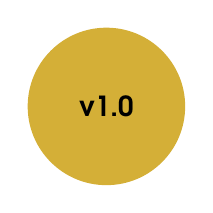
\begin{tikzpicture}
            \fill[fabAccent] (0,0) circle (1cm);
            \node[fabPrimary, font=\bfseries] at (0,0) {v1.0};
        \end{tikzpicture}
        
        \vspace{1cm}
        {\Large\textcolor{fabDark}{May 2025}}
    \end{center}
\end{titlepage}

% Table of contents
\pagenumbering{gobble}
\tableofcontents
\clearpage

\pagenumbering{arabic}

% Main content
\section{Executive Summary}
\fabSectionrule
% Executive Summary - One Page Version
\vspace{0.3cm}
\begin{center}
\textcolor{fabPrimary}{\Large\textbf{Building the Future of Smart Device Creation}}
\end{center}

\vspace{0.2cm}
\noindent !Forge democratizes smart device creation through AI and blockchain technology. Our platform transforms ideas into physical reality without requiring engineering expertise, opening the \$500B+ smart device market to everyone.

\vspace{0.2cm}
\begin{multicols}{2}
\textcolor{fabPrimary}{\textbf{Our Mission}}\\
\noindent To eliminate barriers in hardware creation by providing an intuitive, AI-guided process that anyone can use to build custom smart devices—from drones to automated systems.

\columnbreak

\textcolor{fabPrimary}{\textbf{Market Opportunity}}\\
\noindent \$500B+ smart device market (2025) with 15-30\% growth across IoT sectors. Rising demand for customized devices and growth of maker movement.
\end{multicols}

\vspace{0.2cm}
\begin{multicols}{2}
\textcolor{fabSecondary}{\textbf{Key Platform Features}}
\vspace{0.05cm}
\begin{itemize}[leftmargin=*, topsep=0pt, itemsep=0pt]
    \item AI-guided component selection
    \item Automated code generation
    \item 3D modeling optimization
    \item Decentralized marketplace
    \item Local manufacturing network
\end{itemize}

\columnbreak

\textcolor{fabAccent}{\textbf{Competitive Edge}}
\vspace{0.05cm}
\begin{itemize}[leftmargin=*, topsep=0pt, itemsep=0pt]
    \item End-to-End Solution: Concept to finished device
    \item AI Integration: Simplifies complex processes
    \item Blockchain Utility: Deflationary token mechanics
    \item Network Effects: Value grows with ecosystem
\end{itemize}
\end{multicols}

\vspace{0.2cm}
\begin{center}
\begin{minipage}{0.95\textwidth}
\textcolor{fabSecondary}{\textbf{FRGE Token Ecosystem}}
\end{minipage}
\end{center}

\vspace{0.05cm}
\noindent Our two-tier system offers free users data monetization while premium users pay for privacy. 20\% of subscription revenue buys and burns FRGE tokens, creating deflationary pressure. Marketplace transactions in FRGE enjoy reduced fees (5\% vs 15\% for FIAT), with all FRGE fees burned.

\vspace{0.2cm}
\begin{multicols}{3}
\textcolor{fabPrimary}{\textbf{Token Utility}}
\begin{itemize}[leftmargin=*, topsep=0pt, itemsep=0pt]
    \item Project investment
    \item Data monetization
    \item Marketplace purchases
    \item Professional services
\end{itemize}

\columnbreak

\textcolor{fabSecondary}{\textbf{Distribution}}
\begin{itemize}[leftmargin=*, topsep=0pt, itemsep=0pt]
    \item Investors: 40\%
    \item Team: 20\%
    \item Ecosystem: 20\%
    \item Liquidity: 20\%
\end{itemize}

\columnbreak

\textcolor{fabAccent}{\textbf{Economics}}
\begin{itemize}[leftmargin=*, topsep=0pt, itemsep=0pt]
    \item Total Supply: 100M FRGE
    \item Deflationary model
    \item 20\% of FIAT buys \& burns
    \item All fees burn FRGE
\end{itemize}
\end{multicols}

\vspace{0.2cm}
\noindent The !Forge platform uniquely combines AI, blockchain, and manufacturing to democratize creation capabilities previously available only to large companies and experienced engineers, while establishing a sustainable ecosystem for all participants. 

\clearpage
\section{Market Opportunity}
\fabSectionrule
\subsection{Vision}
To democratize smart device creation, making it accessible to everyone while building a sustainable ecosystem of creators, developers, and manufacturers.

\subsection{Market Landscape}
The smart device market is experiencing unprecedented growth, driven by:
\begin{itemize}[leftmargin=*]
    \item Increasing demand for customized IoT solutions
    \item Growing maker community and DIY culture
    \item Advancements in AI and manufacturing technologies
    \item Rising need for rapid prototyping
\end{itemize}

\subsection{Market Pain Points}
Current challenges in the smart device creation space:
\begin{itemize}[leftmargin=*]
    \item High technical barriers to entry
    \item Fragmented development tools
    \item Limited access to AI capabilities
    \item Expensive prototyping costs
    \item Complex manufacturing processes
\end{itemize}

\subsection{Market Size}
\begin{itemize}[leftmargin=*]
    \item Smart device market: \$500B+ (2025)
    \item DIY electronics: \$15B+ (15\% CAGR)
    \item 3D printing: \$35B+ (20\% CAGR)
    \item AI services: \$200B+ (30\% CAGR)
\end{itemize} 

\clearpage
\section{The !Forge Solution}
\fabSectionrule
\subsection{AI-Powered Development Platform}
!Forge integrates advanced AI systems to transform hardware creation:
\begin{itemize}[leftmargin=*]
    \item Natural language to technical specification conversion
    \item Intelligent design assistance and optimization
    \item Automated engineering fundamentals
\end{itemize}

\subsection{Blockchain-Enabled Infrastructure}
Our decentralized foundation ensures:
\begin{itemize}[leftmargin=*]
    \item Secure and transparent transactions
    \item Tokenized value exchange
    \item Community-driven governance
\end{itemize}

\subsection{Key Innovations}
\begin{itemize}[leftmargin=*]
    \item \textbf{AI Orchestration System}: Seamlessly coordinates all aspects of device creation
    \item \textbf{Component Compatibility Engine}: Ensures perfect component matching
    \item \textbf{Real-time Simulation Platform}: Instantly validates code before manufacturing
    \item \textbf{Decentralized Marketplace}: Allowing the platform to grow organically and add new features
\end{itemize} 

\clearpage
\section{User Experience}
\fabSectionrule
\subsection{Intuitive Interface}
\begin{itemize}[leftmargin=*]
    \item Natural language input for device specifications
    \item Visual design interface with real-time feedback
    \item Step-by-step guided assembly process
    \item Interactive 3D model viewer
\end{itemize}

\subsection{AI Assistance}
\begin{itemize}[leftmargin=*]
    \item Smart suggestions for component selection
    \item Automated compatibility checking
    \item Automated wiring
    \item Automated code generation
    \item Real-time error detection and correction
    \item Context-aware help system
\end{itemize}

\subsection{Community Support}
\begin{itemize}[leftmargin=*]
    \item Expert consultation marketplace
    \item Project sharing and remixing
    \item Local maker space integration
\end{itemize} 

\clearpage
\section{Marketplace \& Professional Services}
\fabSectionrule
\subsection{AI Model Marketplace}
\begin{itemize}[leftmargin=*]
    \item Trading of specialized AI models
    \item Model performance metrics and ratings
    \item Usage-based pricing
    \item Trading of training data
\end{itemize}

\subsection{Expert Marketplace}
\begin{itemize}[leftmargin=*]
    \item Bounties for problem resolution
    \item Custom development services
    \item Assembly assistance
    \item 3D printing services
\end{itemize}

\subsection{Tools Marketplace}
\begin{itemize}[leftmargin=*]
    \item Simulation plugins
    \item AI prompts
    \item Component libraries
    \item Libraries and code snippets
\end{itemize}

\subsection{3D Models Marketplace}
\begin{itemize}[leftmargin=*]
    \item Ready to print specialized parts
    \item Models of components
    \item Joints and connectors
\end{itemize}

\clearpage
\section{AI Training \& Improvement}
\fabSectionrule
\subsection{Training Data Sources}
\begin{itemize}[leftmargin=*]
    \item User project data (anonymized)
    \item Component specifications and datasheets
    \item Manufacturing guidelines
    \item Expert knowledge base
    \item Simulation results
\end{itemize}

\subsection{Model Architecture}
\begin{itemize}[leftmargin=*]
    \item Multi-modal AI system
    \item Specialized sub-networks
    \item Continuous learning pipeline
    \item Quality assurance mechanisms
    \item Performance monitoring
\end{itemize}

\subsection{Training Process}
\begin{itemize}[leftmargin=*]
    \item Distributed training on Bittensor
    \item Automated hyperparameter optimization
    \item Cross-validation and testing
\end{itemize}

\clearpage
\section{Tokenomics}
\fabSectionrule
\highlightBox{Utility}{
The FAB token is designed as a utility token that primarily serves as an investment vehicle and purchasing power for Fabrikator projects. Unlike traditional utility tokens, FAB is not used for platform fees, governance, or AI service payments.
}

\subsection*{User Tiers and Data Monetization}

Fabrikator offers two user tiers: Free and Premium.

\begin{itemize}[leftmargin=*]
    \item \textbf{\textcolor{fabPrimary}{Free Users:}} Do not pay platform fees. Their project data may be sold by the platform (for FAB tokens) to AI trainers, creating ongoing demand for FAB. Free users pay for AI services in FIAT or TAO and can purchase marketplace content with FIAT or FAB.
    \item \textbf{\textcolor{fabSecondary}{Premium Users:}} Pay a monthly subscription fee in FIAT for enhanced privacy; their project data is neither sold nor used for AI training. Premium users can also purchase marketplace content with FIAT or FAB. Premium users can decide to sell their projects data to earn FAB tokens when their data is used.
\end{itemize}

\subsection*{Token Utility}
\begin{itemize}[leftmargin=*]
    \item \textbf{\textcolor{fabPrimary}{Project Investment \& Purchasing Power:}} FAB tokens provide investors with purchasing power for projects created on the platform, enabling them to acquire projects that can be used to train their AI models
    \item \textbf{\textcolor{fabPrimary}{Project Monetization:}} Premium users can sell their completed projects for FAB tokens
    \item \textbf{\textcolor{fabPrimary}{Bounty Payments:}} FAB tokens can be used to pay for bounties on the platform
    \item \textbf{\textcolor{fabPrimary}{Professional Services:}} Assembly and 3D printing professionals can accept FAB as payment for their services
    \item \textbf{\textcolor{fabPrimary}{Data Purchases:}} AI trainers and providers can purchase project data (from the platform or from premium users) using FAB tokens, creating ongoing demand. \textbf{All FAB earned from data sales is burned by the platform.}
\end{itemize}

\subsection*{Token Distribution}

% Create a custom pie chart for token distribution
\begin{center}
\begin{tikzpicture}[scale=1.3]
    % Define pie chart segments
    \def\radius{2.5}
    
    % Investor slice (40%)
    \fill[fabPrimary] (0,0) -- (0:\radius) arc (0:144:\radius) -- cycle;
    
    % Team slice (20%)
    \fill[fabSecondary] (0,0) -- (144:\radius) arc (144:216:\radius) -- cycle;
    
    % Ecosystem slice (20%)
    \fill[fabAccent] (0,0) -- (216:\radius) arc (216:288:\radius) -- cycle;
    
    % Liquidity slice (20%)
    \fill[fabGrey] (0,0) -- (288:\radius) arc (288:360:\radius) -- cycle;
    
    % Add labels with percentages
    \node[white, font=\bfseries] at (72:\radius*0.7) {Investors: 40\%};
    \node[white, font=\bfseries] at (180:\radius*0.7) {Team: 20\%};
    \node[white, font=\bfseries] at (252:\radius*0.7) {Ecosystem: 20\%};
    \node[white, font=\bfseries] at (324:\radius*0.7) {Liquidity: 20\%};
\end{tikzpicture}
\end{center}

\begin{itemize}[leftmargin=*]
    \item \textbf{\textcolor{fabPrimary}{Investors:}} 40\% - For project investment and purchasing power
    \item \textbf{\textcolor{fabSecondary}{Team \& Development:}} 20\% - Vesting over 3 years
    \item \textbf{\textcolor{fabAccent}{Ecosystem Growth:}} 20\% - For platform development and community incentives
    \item \textbf{\textcolor{fabGrey}{Liquidity Pool:}} 20\% - For FAB/TAO liquidity
\end{itemize}

\subsection*{Payment Model}

\highlightBox{Core Payment Systems}{
\begin{itemize}[leftmargin=*]
    \item \textbf{\textcolor{fabPrimary}{FAB Token:}}
    \begin{itemize}
        \item Used to purchase project data (from the platform or from premium users), marketplace content, and professional services.
        \item Demand is created by AI trainers and marketplace participants.
        \item 20\% of FIAT income from premium subscriptions is used to buy and burn FAB, creating a deflationary mechanic.
    \end{itemize}
    \item \textbf{\textcolor{fabSecondary}{TAO (Bittensor's native token):}}
    \begin{itemize}
        \item Used for all AI-related services, including model training and inference.
    \end{itemize}
    \item \textbf{\textcolor{fabGrey}{FIAT Currency:}}
    \begin{itemize}
        \item Used for premium subscriptions, AI services, and marketplace purchases.
        \item 20\% of premium subscription income is used to buy and burn FAB.
    \end{itemize}
\end{itemize}
}

\vspace{1em}

\begin{itemize}[leftmargin=*]
    \item \textbf{\textcolor{fabAccent}{Liquidity:}}
    \begin{itemize}
        \item Liquidity is provided for FAB/TAO trading pairs to ensure smooth conversion between tokens and to support a healthy marketplace.
    \end{itemize}
    \item \textbf{\textcolor{fabPrimary}{Marketplace Fees:}}
    \begin{itemize}
        \item All marketplace transactions incur a 15\% platform fee if they are performed in FIAT.
        \item All marketplace transactions incur a 5\% platform fee if they are performed in FAB. \textbf{This 5\% fee is used to burn FAB, creating additional deflationary pressure.}
    \end{itemize}
\end{itemize}

\subsection*{Token Economics}
\begin{itemize}[leftmargin=*]
    \item \textbf{\textcolor{fabPrimary}{Total Supply:}} 100,000,000 FAB
    \item \textbf{\textcolor{fabSecondary}{Raising:}} 20,000 TAO (approximately \$8,770,000 at \$438.50 per TAO)
\end{itemize}

\subsection*{Deflationary Mechanism}

\highlightBox{Deflationary Strategy}{
To ensure long-term value and scarcity, 20\% of all FIAT income from premium subscriptions is used by the platform to purchase FAB tokens on the open market, which are then permanently burned. Additionally, the 5\% fee collected from all marketplace transactions performed in FAB is also burned, and all FAB earned from data sales to AI trainers is burned, further increasing the deflationary effect and buy pressure on FAB.
}

\subsection*{Use of Funds}
The funds raised and generated through the Fabrikator platform are allocated as follows:
\begin{itemize}[leftmargin=*]
    \item \textbf{\textcolor{fabPrimary}{20\%}} of premium subscription FIAT income is used to buy and burn FAB tokens.
    \item \textbf{\textcolor{fabSecondary}{80\%}} of premium subscription FIAT income goes to the treasury for platform maintenance, scaling, AI model training, and potential buyouts of successful marketplace models.
    \item \textbf{\textcolor{fabAccent}{Marketplace Fees:}} 5-15\% platform fee is taken from all marketplace transactions.
    \item \textbf{\textcolor{fabGrey}{Other allocations:}} Funds may also be used for marketing, community growth, and ecosystem partnerships as needed.
\end{itemize}

These allocations are designed to maximize platform growth, user adoption, and long-term sustainability.

% --- Improved Projected Income Section ---

\subsection*{Projected Income}

\highlightBox{Monthly Income \& FAB Burning Projections}{
To illustrate the platform's earning potential and the resulting FAB buy and burn pressure, we project monthly income and FAB demand as the user base grows from 1 to 20,000 users. The following assumptions are used:

\begin{itemize}[leftmargin=*]
    \item 1 in 7 users is a premium user (\textasciitilde14.3\%), 6 in 7 are free users.
    \item Premium monthly fee: \$150.
    \item All users spend \$50/month on AI usage (platform takes 15\% fee).
    \item All users spend \$20/month on the marketplace in FIAT (15\% fee) and \$5/month in FAB (5\% fee, \textbf{all of which is burned}).
    \item 20\% of premium FIAT income is used to buy and burn FAB.
    \item \textbf{AI trainers purchase data for \$1/month in FAB per free user} (\textasciitilde6/7 of total users), \textbf{all of which is burned by the platform}.
\end{itemize}
}

\textbf{\textcolor{fabPrimary}{Formulas:}}

\begin{itemize}[leftmargin=*]
    \item Premium users: $N_{\text{premium}} = \frac{N_{\text{total}}}{7}$
    \item Free users: $N_{\text{free}} = N_{\text{total}} \times \frac{6}{7}$
    \item FIAT income from premiums: $I_{\text{premium}} = N_{\text{premium}} \times 150$
    \item AI usage fee income: $I_{\text{AI}} = N_{\text{total}} \times 50 \times 0.15$
    \item Marketplace FIAT fee: $I_{\text{mkt,FIAT}} = N_{\text{total}} \times 20 \times 0.15$
    \item Marketplace FAB fee (burned): $I_{\text{mkt,FAB}} = N_{\text{total}} \times 5 \times 0.05$
    \item \textbf{Total FIAT income:} $I_{\text{FIAT,tot}} = I_{\text{premium}} + I_{\text{AI}} + I_{\text{mkt,FIAT}}$
    \item \textbf{FIAT used to buy and burn FAB:} $B_{\text{FAB,FIAT}} = I_{\text{premium}} \times 0.2$
    \item \textbf{FAB burned (marketplace + data):} $B_{\text{FAB,direct}} = I_{\text{mkt,FAB}} + N_{\text{free}}$
    \item \textbf{Total FAB burned:} $B_{\text{FAB,tot}} = B_{\text{FAB,FIAT}} + B_{\text{FAB,direct}}$
\end{itemize}

\begin{center}
\begin{tikzpicture}[scale=1.1]
    % Set modern style
    \pgfplotsset{
        every axis/.append style={
            line width=1.5pt,
            tick style={color=fabDark},
            label style={font=\bfseries},
            title style={font=\bfseries},
            grid=both,
            grid style={line width=.1pt, draw=fabGrey!10},
            major grid style={line width=.2pt,draw=fabGrey!25},
            axis lines=middle,
            every axis grid/.style={fabGrey},
            width=\textwidth-2cm,
            height=7cm
        }
    }
    
    % Define the axes
    \begin{axis}[
        xlabel={\textbf{Users (thousands)}},
        ylabel={\textbf{Monthly USD (thousands)}},
        xmin=0, xmax=10.5,
        ymin=0, ymax=8.5,
        xtick={0,2,4,6,8,10},
        xticklabels={0,5,10,15,20,25},
        ytick={0,2,4,6,8},
        yticklabels={0,100,200,300,400},
        legend style={
            at={(0.5,-0.28)},
            anchor=north,
            font=\footnotesize\sffamily,
            cells={anchor=west},
            draw=none,
            legend columns=2
        },
    ]
    
    % Plot FIAT income from premium subscriptions
    \addplot[color=fabPrimary, thick, mark=*] coordinates {
        (0,0) (2,0.8) (4,1.6) (6,2.4) (8,3.2) (10,4.0)
    };
    
    % Plot FIAT income from AI usage fees
    \addplot[color=fabSecondary, thick, mark=square*] coordinates {
        (0,0) (2,0.9) (4,1.8) (6,2.7) (8,3.6) (10,4.5)
    };
    
    % Plot FIAT income from marketplace fees
    \addplot[color=fabAccent, thick, mark=triangle*] coordinates {
        (0,0) (2,0.4) (4,0.8) (6,1.2) (8,1.6) (10,2.0)
    };
    
    % Plot Corrected Total FAB burning (with correct calculation)
    \addplot[color=fabSecondary, thick, mark=diamond*, dashed] coordinates {
        (0,0) (2,0.54) (4,1.08) (6,1.62) (8,2.16) (10,2.7)
    };
    
    % Legend
    \legend{Premium Subscriptions, AI Usage Fees, Marketplace FIAT Fees, Total FAB Burned};
    \end{axis}
\end{tikzpicture}
\end{center}

\vspace{1.5cm}

% Key points from table
\begin{center}
\begin{tcolorbox}[
    colframe=fabPrimary,
    colback=fabLight,
    boxrule=1pt,
    title=\textbf{Monthly Projections at Different User Levels},
    fonttitle=\bfseries\sffamily\color{white},
    left=6pt,
    right=6pt,
    top=6pt,
    bottom=6pt,
    width=\textwidth-0.5cm
]
\renewcommand{\arraystretch}{0.9}
\begin{tabular}{|c|c|c|c|c|}
\hline
\textbf{Users} & \textbf{Premium Users} & \textbf{Free Users} & \textbf{Monthly FIAT} & \textbf{Monthly FAB Burned} \\
\hline
1,000 & 143 & 857 & \$21,428 & \$5,397 \\
\hline
5,000 & 714 & 4,286 & \$107,143 & \$26,956 \\
\hline
10,000 & 1,429 & 8,571 & \$214,286 & \$53,941 \\
\hline
25,000 & 3,571 & 21,429 & \$535,714 & \$134,815 \\
\hline
\end{tabular}
\end{tcolorbox}
\end{center}

\highlightBox{Notes}{
\begin{itemize}[leftmargin=*]
    \item \textbf{Total FIAT Income} includes premium subscriptions, AI usage fees, and marketplace FIAT fees.
    \item \textbf{FIAT Used to Buy \& Burn FAB} is the amount of FIAT from premium subscriptions used monthly to buy and burn FAB (20\%).
    \item \textbf{FAB Burned (Marketplace + Data)} includes the 5\% fee on marketplace FAB transactions plus the \$1 per free user from data sales.
    \item \textbf{Monthly FAB Burned} is the total of all FAB burning mechanisms combined.
    \item At 20,000 users, approximately \$108,000 worth of FAB is burned monthly.
\end{itemize}
} 

\clearpage
\section{Roadmap}
\fabSectionrule
\subsection{Q4 2025: Fundraising}
\begin{itemize}[leftmargin=*]
    \item Core team assembly
    \item Platform architecture design
    \item Initial token distribution
    \item Proof of concept
    \item Initial marketing campaign
\end{itemize}

\subsection{Q3 2026: Core Features}
\begin{itemize}[leftmargin=*]
    \item Alpha version of the platform
    \item Integration with Bittensor marketplace
    \item Beginning of training data collection
    \item Agressive marketing campaign
\end{itemize}

\subsection{Q1 2027: Custom AI models}
\begin{itemize}[leftmargin=*]
    \item Integration of other AI platforms
    \item Integration with Bittensor marketplace
    \item Training of custom AI models
\end{itemize}

\subsection{Q2 2027: Release & Marketplace}
\begin{itemize}[leftmargin=*]
    \item Official release of the building platform
    \item Introduction of the marketplace
    \item Users can select AI models from the marketplace
\end{itemize}

\subsection{Q3 2027: Professional Services}
\begin{itemize}[leftmargin=*]
    \item Bounties
    \item Assembly and 3D printing services added to marketplace
\end{itemize}


\clearpage
\section{Conclusion}
\fabSectionrule
\vspace{0.5cm}
\noindent !Forge represents a paradigm shift in smart device creation, combining cutting-edge AI technology with blockchain innovation to democratize access to custom device development. Our platform eliminates technical barriers while fostering a sustainable ecosystem of creators, developers, and manufacturers.

\vspace{0.5cm}
\noindent\textbf{Key Takeaways:}
\begin{itemize}[leftmargin=*]
    \item Revolutionary AI-powered development platform
    \item Decentralized marketplace for components and services
    \item Strong focus on community and sustainability
    \item Clear roadmap for growth and development
\end{itemize}

\vspace{0.5cm}
\noindent\textbf{Next Steps:}
\begin{itemize}[leftmargin=*]
    \item Launch of initial platform features
    \item Community building and engagement
    \item Strategic partnership development
    \item Token generation event
\end{itemize}

\end{document} 